\begin{figure*}[t!]
    \centering
    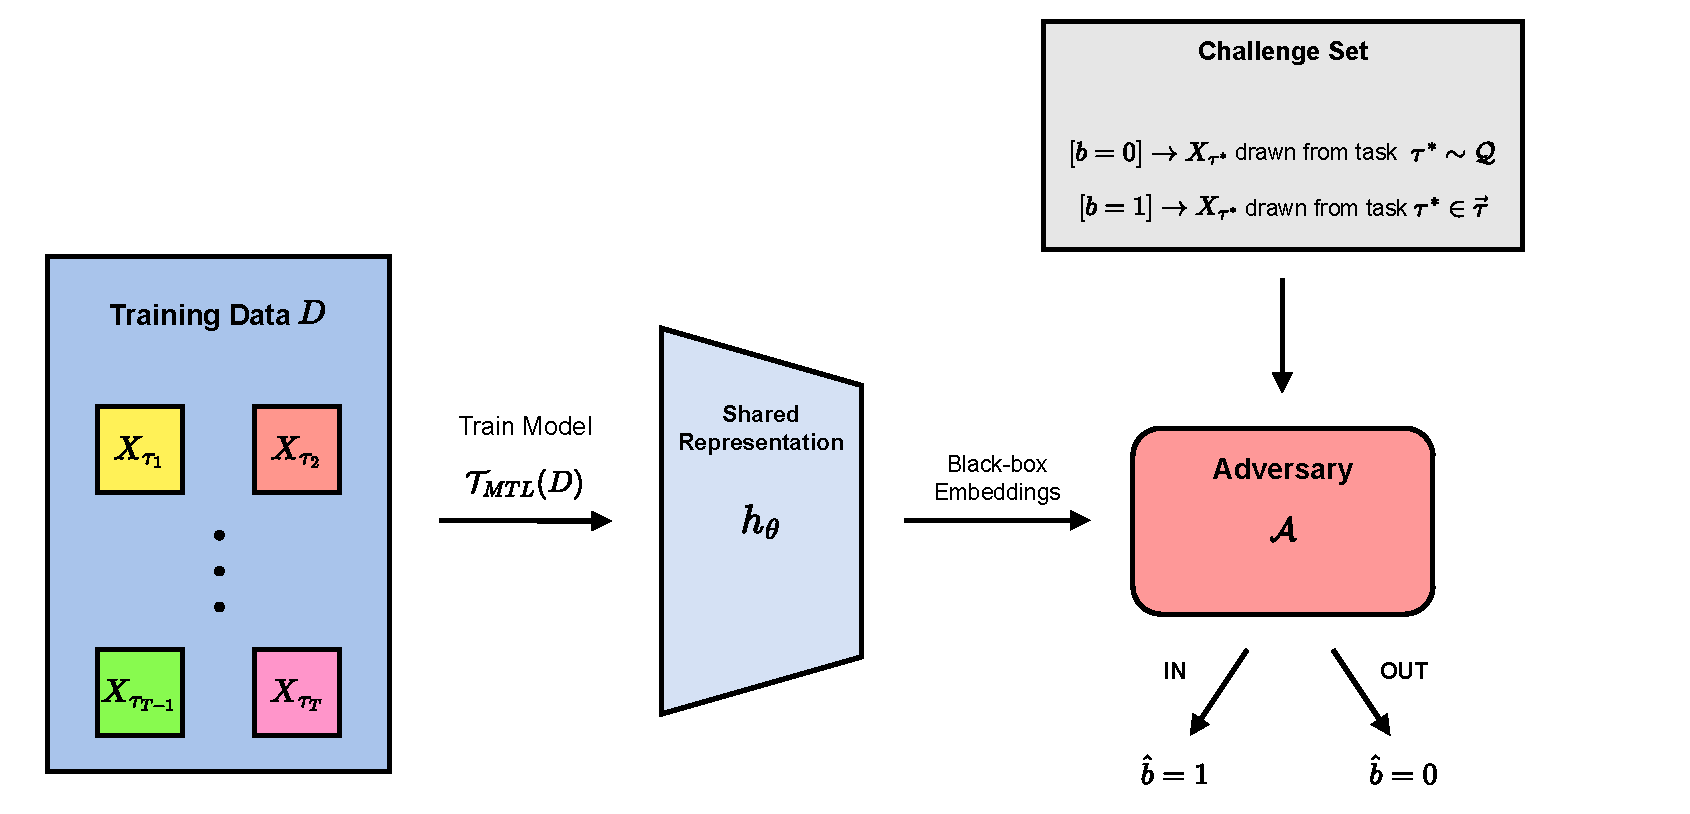
\includegraphics[width=0.8\linewidth]{figs/threat-model.pdf}
    \caption{Security Game for Task Inference Attacks}
    \label{fig:threat-model}
\end{figure*}

\section{Threat Model} \label{sec:threatmodel}


Our goal is to assess whether shared representations reveal information about the specific tasks that they were trained on and to what degree they reveal this information. Towards this, we study privacy leakage in shared representations through the lens of inference attacks~\cite{homer-2008-mi, shokri-2016-mi, ateniese-2015-property_inference}. In this setting, there is an MTL model that is trained on several tasks simultaneously to learn a shared representation, or encoder, and individual task layers. Queries can then be made to the encoder to receive representation vectors, or embeddings, for any given input. A challenge task is drawn from the same distribution as the tasks used to train the MTL model. Our adversary uses their query access to the shared representation, along with data drawn from the challenge task, to infer whether the challenge task was included while training the MTL model. In this work, we study this leakage from a purely black-box perspective, only assuming query access and no knowledge of the underlying task distribution to train shadow models as is common in prior works~\cite{carlini-2022-lira}. Additionally, we reveal a separation between a \emph{strong adversary} that receives a set of the actual training data from the challenge task, and a \emph{weak adversary} that receives non-training data drawn from the same distribution as the challenge task. We can describe our threat model using the following security game between a \textit{challenger} and an \textit{adversary}:

 % \noindent \textbf{Task Inference Security Game} 

 % [See also version in main.tex]


% \subsection{Security game}

% \begin{defn} (Needs reformatting)
    
%     \noindent Given: 

% - target task $\tau^*$

% - distribution $\mathcal{Q}$ on task sets  of size $n$ (not necessarily i.i.d.)

% - learning algorithm which outputs an ``encoder'' $h$. 

% - bit $b$

% - attacker algorithm

% \noindent 
% Experiment: 

% - Select $\vec\tau = \tau_1,...,\tau_n$ from $\mathcal{Q}$

% - Generate data $\vec{\mathcal{X}} =\mathcal{X}_1,...,\mathcal{X}_n$ from tasks in $\vec \tau$

% - If $b=1$ (IN) then set $\vec{\mathcal{X}} = (\mathcal{X}^*,\mathcal{X}_2,...,\mathcal{X}_n)$

% - Run learner on $\mathcal{X}_1,...,\mathcal{X}_n$ to get $h$

% - Run attack on $h, \tau^*, \mathcal{T}$ to get bit $\hat b$. Strong attacker also gets $\mathcal{X^*}$

% - Attacker wins if $\hat b=b$
% \end{defn}

 \begin{enumerate}[labelsep=*,leftmargin=15pt]
     \item[]  \begin{center}
         \textbf{Task Inference Security Game}
     \end{center} 
     \item The challenger receives $T$ tasks $\vec{\tau} = ( \tau_1, \dots, \: \tau_T )$, drawn from a task distribution $\mathcal{Q}$. For each of the tasks, $\tau_i$, the challenger is given a batch of samples $X_i$ and concatenates the $T$ batches into a dataset $D = \{X_{\tau_1}, \dots, X_{\tau_T} \}$.
     \item The challenger trains a \textit{shared representation} $h_\theta~\gets~\mathcal{T}_{\mathit{MTL}}(D)$ by simultaneously learning \emph{task-specific} models that share $h_\theta$.
     \item The challenger randomly selects $b \in \{0, 1\}$. If  $b = 0$, the challenger samples a challenge task $\tau^*$ from $\mathcal{Q}$ uniformly at random, such that $\tau^* \notin \vec{\tau}$. Otherwise, the challenger samples $\tau^*$ from $\vec{\tau}$ uniformly at random. 
     \item The challenger sends a batch of samples, $X^*$, drawn from the challenge task, $\tau^*$.
     \item The adversary, using the batch of samples and black-box access to $h_\theta$, guesses a bit $\hat{b} \gets \mathcal{A}(h_\theta(X_{\tau^*}))$.
     \item The adversary wins if $\hat{b} = b$ and loses otherwise.
 \end{enumerate}

In this security game the adversary only requires samples drawn from the challenge task rather than the specific training samples from $D$. We claim that a task-inference adversary does not necessarily need data from a member of the training dataset to perform an inference attack on a task that contains their data. Semantically, if a multitask model is trained over sparse data from several tasks, our proposed adversary can use \textit{fresh data} from a given task's data distribution to infer whether the task was included in the training dataset. We use the following terms to define this distinction: A task-inference adversary is \textbf{strong} if they have access to training samples when $b=1$ or \textbf{weak} if they \emph{do not} have access to training samples when $b=1$. In either setting, a task-inference adversary can mount attacks to infer inclusion of a task in training. To support this claim, we show a separation between the \textbf{strong} and \textbf{weak} adversaries in Section~\ref{sec:mean_est} and empirically verify this separation in Section~\ref{sec:eval}. 

Our proposed threat model interpolates those of existing property existence attacks~\cite{chaudhari-2022-snap} and user inference attacks~\cite{kandpal2023userinference}. Suppose that the challenger trains a MTL model over many users, such that each task belongs to a unique user.  In this setting, the adversary is distinguishing between worlds where a MTL model was or was not trained on a specific user's data. Detecting the inclusion of a task in MTL training yields the same privacy violation as user inference. If the task only includes one sample per user, the attack reduces to membership inference where each sample belongs to a member. When MTL is used to train tailored classifiers for multiple learning problems, each with limited data, our task-inference adversary is distinguishing between worlds where the model was or was not trained on a particular pair of samples and labels. In other words, the adversary is attempting to determine if samples that satisfy the labeling for a given task were included in MTL training. Here, we can think of tasks as properties or distributions within the training dataset since the inclusion or noninclusion of a task determines whether or not a particular distribution of labels over samples was learned during MTL training. Thus, inferring the inclusion of a task yields a similar privacy violation to property existence~\cite{chaudhari-2022-snap}, where an adversary can determine the subpopulations that compose the dataset. 


Additionally, we note that the adversary described in the security game operates in a black-box manner, only requiring query access to the representation $h_\theta$. In contrast to prior work on membership and property inference, our adversary \emph{does not} require shadow models nor sampling access to the underlying data distribution~\cite{carlini-2022-lira, mahloujifar2022propertypoisoning,shokri-2016-mi, liu2021encodermi, abascal2023tmi}. Our task-inference adversary's access can be viewed as similar to that of the membership inference adversary described in \cite{liu2021encodermi}. In this work, the adversary makes black-box queries to a representation model and receives embedding vectors for multiple correlated samples which are then used to mount an attack. In contrast, the adversary proposed by~\citet{liu2021encodermi} also makes black-box queries to the shared representation but has access to additional samples from the training data distribution to train shadow models, whereas we assume pure black-box access.